
%(BEGIN_QUESTION)
% Copyright 2011, Tony R. Kuphaldt, released under the Creative Commons Attribution License (v 1.0)
% This means you may do almost anything with this work of mine, so long as you give me proper credit

Identify the pressure readings one would expect to see on the two gauges of this positioner at the following pneumatic signal values, assuming proper signal-to-open calibration:

$$\includegraphics[width=15.5cm]{i01401x01.eps}$$

\begin{itemize}
\item{} Gauge readings at 0\% (3 PSI) signal to the positioner
\item{} Gauge readings at 50\% (9 PSI) signal to the positioner
\item{} Gauge readings at 100\% (15 PSI) signal to the positioner
\end{itemize}

Finally, identify what these gauges would indicate if the valve were seized in the mid-open (50\%) position due to excessive packing friction, assuming the pneumatic input signal was at 9.4 PSI.

\underbar{file i01401}
%(END_QUESTION)





%(BEGIN_ANSWER)

\begin{itemize}
\item{} Gauge readings at 0\% (3 PSI) signal to the positioner: {\it left-hand gauge saturated high (full pressure), right-hand gauge saturated low (0 PSI)}
\item{} Gauge readings at 50\% (9 PSI) signal to the positioner: {\it too little information to given to tell.  We would have to know the valve's bench set pressure range as well as any other forces acting on the stem such as packing friction}
\item{} Gauge readings at 100\% (15 PSI) signal to the positioner: {\it left-hand gauge saturated low (0 PSI), right-hand gauge saturated high (full pressure)}
\end{itemize}

%(END_ANSWER)





%(BEGIN_NOTES)

In the seized scenario, the positioner would saturate to drive the valve open more: no pressure on the left-hand gauge and full pressure on the right-hand gauge.

\vskip 20pt \vbox{\hrule \hbox{\strut \vrule{} {\bf Virtual Troubleshooting} \vrule} \hrule}

This question is a good candidate for a ``Virtual Troubleshooting'' exercise.  Presenting the diagram to students, you first imagine in your own mind a particular fault in the system.  Then, you present one or more symptoms of that fault (something noticeable by an operator or other user of the system).  Students then propose various diagnostic tests to perform on this system to identify the nature and location of the fault, as though they were technicians trying to troubleshoot the problem.  Your job is to tell them what the result(s) would be for each of the proposed diagnostic tests, documenting those results where all the students can see.

During and after the exercise, it is good to ask students follow-up questions such as:

\begin{itemize}
\item{} What does the result of the last diagnostic test tell you about the fault?
\item{} Suppose the results of the last diagnostic test were different.  What then would that result tell you about the fault?
\item{} Is the last diagnostic test the best one we could do?
\item{} What would be the ideal order of tests, to diagnose the problem in as few steps as possible?
\end{itemize}

%INDEX% Final Control Elements, valve: positioner

%(END_NOTES)


